\documentclass[aspectratio=169, 11pt]{beamer}

% --- Packages & Setup (template set, plus lmodern so code text is vector, not bitmap) ---
\usepackage[utf8]{inputenc}
\usepackage[T1]{fontenc}
\usepackage{lmodern}
\usepackage{helvet}
\renewcommand{\familydefault}{\sfdefault}
\usepackage{xcolor}
\usepackage{booktabs}
\usepackage{graphicx}
\usepackage{array}
\usepackage{adjustbox}
\usepackage{tikz}
\usetikzlibrary{calc, positioning, arrows.meta, fit}

\graphicspath{{./}{../figures/}}

% --- Branding Colors ---
\definecolor{amritaMaroon}{HTML}{A4123F}
\definecolor{tierFill}{HTML}{FBEFF3}
\definecolor{dataFill}{HTML}{EEF6F5}
\definecolor{offFill}{HTML}{FDF7EC}
\definecolor{okGreen}{HTML}{1E7B34}

% --- Theme Setup ---
\usetheme{Madrid}
\usecolortheme[named=amritaMaroon]{structure}
\setbeamertemplate{navigation symbols}{}
\setbeamertemplate{footline}[frame number]
\setbeamertemplate{itemize items}[circle]
\setlength{\leftmargini}{1.2em}

\newcolumntype{L}[1]{>{\raggedright\arraybackslash}p{#1}}
\newcommand{\ok}{\textcolor{okGreen}{\textbf{Done}}}

% Shared TikZ styles for every diagram in the deck.
\tikzset{
  box/.style={draw=amritaMaroon, fill=tierFill, rounded corners=2pt, align=center, inner sep=2.5pt, font=\sffamily\scriptsize},
  dbox/.style={draw=teal!70!black, fill=dataFill, rounded corners=2pt, align=center, inner sep=2.5pt, font=\sffamily\scriptsize},
  obox/.style={draw=orange!70!black, fill=offFill, rounded corners=2pt, align=center, inner sep=2.5pt, font=\sffamily\scriptsize},
  tier/.style={draw=amritaMaroon, rounded corners=3pt, inner sep=4pt},
  lbl/.style={font=\sffamily\bfseries\scriptsize, text=amritaMaroon, anchor=south west},
  arr/.style={-{Stealth[length=1.6mm]}, thick, draw=black!65},
  ent/.style={draw=amritaMaroon, fill=white, rounded corners=2pt, align=left, inner sep=3pt, font=\sffamily\scriptsize, text width=3.9cm, execute at begin node={\hyphenpenalty=10000}},
}

\begin{document}

% =========================================================================
% TITLE SLIDE (Software-Based Project)
% =========================================================================
\begin{frame}
    \begin{tikzpicture}[remember picture,overlay]
        \node[fill=amritaMaroon, text=white, font=\bfseries\footnotesize, anchor=north east, rounded corners=2pt, inner sep=5pt]
        at ($(current page.north east) + (-0.2cm,-0.2cm)$)
        {Type 3: Software Project};
    \end{tikzpicture}

    \centering
    
\includegraphics[width=2.8cm]{logo.png}
    \vspace{0.1cm}

    {\large \textbf{\textcolor{amritaMaroon}{Real-Time Adaptive Cross-Media Recommendation System}}} \\
    {\footnotesize \textcolor{amritaMaroon}{A domain-agnostic engine with audience eligibility}} \\
    \vspace{0.05cm}
    {\footnotesize \textbf{23CSE498 -- Project Phase II (External Review)} \quad | \quad \textbf{Team Number: G022}} \\
    \vspace{0.12cm}

    \begin{table}
        \centering
        \footnotesize
        \renewcommand{\arraystretch}{1.05}
        \begin{tabular}{|c|c|l|}
            \hline
            \textbf{S.No} & \textbf{Register Number} & \textbf{Student Name} \\
            \hline
            1 & CB.SC.U4CSE23051 & Sanjay A. K. \\
            \hline
            2 & CB.SC.U4CSE23022 & Eswara Raj M. \\
            \hline
            3 & CB.SC.U4CSE23324 & Aditya Vijay \\
            \hline
            4 & CB.SC.U4CSE23359 & Himaneesh Reddy Jangalapalli \\
            \hline
        \end{tabular}
    \end{table}
    \vspace{0.05cm}

    {\scriptsize Guides: \textbf{Dr. Bagavathi Sivakumar P.}, Associate Professor \& Chairperson, School of Computing \\
    \textbf{Dr. Krishna Priya G.}, Assistant Professor (OC), Department of CSE} \\
    \vspace{0.08cm}
    {\scriptsize 16 November 2026}
\end{frame}

% =========================================================================
% PROJECT TITLE & PROBLEM STATEMENT
% =========================================================================
\begin{frame}{Project Title \& Problem Statement}
    \framesubtitle{What we built, and why existing recommenders fall short}
    \begin{block}{Project Title}
        \centering
        \textbf{Real-Time Adaptive Cross-Media Recommendation System}\\
        {\footnotesize A domain-agnostic engine with audience eligibility, across 7 content types}
    \end{block}
    \begin{columns}[T]
        \column{0.49\textwidth}
        \begin{block}{Problem Statement}
            \scriptsize
            Users describe what they want in their own words, across very different kinds of items. Existing recommenders:
            \begin{itemize}
                \item serve \textbf{one domain} only, so one query cannot reach films, books, music and products together;
                \item need \textbf{interaction history}, so a new user gets nothing useful (cold start);
                \item apply age and safety rules \textbf{after ranking}, where ineligible items can leak back onto the page;
                \item adapt only by \textbf{retraining}, and do not say \textbf{why} an item was recommended.
            \end{itemize}
        \end{block}
        \column{0.49\textwidth}
        \begin{block}{Objectives}
            \scriptsize
            \begin{itemize}
                \item \textbf{One engine, 4 domains:} 120,747 items, 7 content types, searched by meaning and by name.
                \item \textbf{Works from the first query:} semantic search needs no history.
                \item \textbf{Safe by construction:} age, safe mode and risk tier filter \emph{inside} the search; 0 violations.
                \item \textbf{Adapts and explains:} every click updates the next search, and every result shows its score breakdown and a knowledge-graph reason.
            \end{itemize}
        \end{block}
    \end{columns}
\end{frame}

% =========================================================================
% GUIDE APPROVAL (Mandatory)
% =========================================================================
\begin{frame}{Guide Review \& Submission Approval}
    \framesubtitle{Confirmation of Project Review and Approval from Guide}
    \centering
    % Save the screenshot as guide_approval.png in this folder and rebuild; it then replaces the box.
    \IfFileExists{guide_approval.png}{%
        \includegraphics[width=0.94\textwidth, height=5.6cm, keepaspectratio]{guide_approval.png}%
    }{%
    \fbox{\begin{minipage}[c][5.4cm]{0.94\textwidth}
        \centering
        \textbf{\textcolor{red}{[Insert Screenshot of Guide Approval Email Here]}} \\[0.3cm]
        {\footnotesize Save it as \texttt{guide\_approval.png} next to this file and rebuild.}
    \end{minipage}}}
\end{frame}

% =========================================================================
% PREVIOUS REVIEW
% =========================================================================
\begin{frame}{Previous Review: Recommendations and What We Did}
    \framesubtitle{Both panel recommendations are delivered and measured}
    \footnotesize
    \renewcommand{\arraystretch}{1.3}
    \begin{tabular}{L{3.3cm} L{8.9cm} c}
        \toprule
        \textbf{Recommendation} & \textbf{What we did} & \textbf{Status} \\
        \midrule
        \textbf{1. Try Neural Collaborative Filtering (NCF)} &
        Implemented NeuMF (GMF + MLP) in PyTorch and benchmarked it on the \emph{same} split as LightGCN on two Amazon domains. It beats LightGCN as the paper scores it (cosine), but LightGCN scored by its trained dot product beats NeuMF by \textbf{1.32$\times$} and \textbf{1.42$\times$} (Recall@20). & \ok \\
        \textbf{2. Age-based content filtering} &
        Six-level maturity ladder, safe mode, risk tiers and domain packs, compiled \emph{into} the vector search. \textbf{0 violations} in the top 20 for every viewer profile. & \ok \\
        \bottomrule
    \end{tabular}

    \vspace{0.3cm}
    \begin{block}{Also added since the last review}
        \scriptsize
        Email and Google accounts with onboarding and self-service deletion $\cdot$ typo correction and a nonsense-query gate $\cdot$ connection pooling (4.6$\times$ faster reads) $\cdot$ login lockout that survives restarts $\cdot$ one-command deployment $\cdot$ CI on every push $\cdot$ \textbf{typed knowledge graph} with explanations $\cdot$ two ranking bugs fixed $\cdot$ tests \textbf{326 $\rightarrow$ 390} $\cdot$ paper \textbf{accepted at ICMLDE 2026}
    \end{block}
\end{frame}

% =========================================================================
% SECTION 1: SRS
% =========================================================================
\section{SRS, Architecture \& Design}

\begin{frame}{1. Software Requirements Specification (SRS)}
    \framesubtitle{System Scope, Primary Actors, Use Cases \& Requirements}
    \begin{columns}[T]
        \column{0.47\textwidth}
        \begin{block}{System Scope \& Core Use Cases}
            \scriptsize
            \begin{itemize}
                \item \textbf{Scope:} one engine for \textbf{120,747 items} in 4 domains; a new domain is a YAML entry. Health and finance are \emph{discovery only}, with advisories.
                \item \textbf{Actors:} visitor (13 demo personas), registered user, guardian (safe mode), data engineer (offline pipeline), external APIs.
                \item \textbf{Use cases:} search \& recommend $\cdot$ give feedback and see results adapt $\cdot$ audience-safe browsing $\cdot$ account sign-up, onboarding, deletion.
            \end{itemize}
        \end{block}
        \column{0.51\textwidth}
        \begin{block}{Functional Requirements}
            \scriptsize
            \begin{itemize}
                \item \textbf{FR-1:} free-text hybrid retrieval (creator, title, semantic) with typo correction.
                \item \textbf{FR-2:} eligibility (age, safe mode, domain, risk) enforced \emph{inside} retrieval.
                \item \textbf{FR-3:} every interaction updates the user's taste immediately, no retraining.
                \item \textbf{FR-4:} per-signal score explanation; \textbf{FR-5:} accounts and data deletion.
            \end{itemize}
        \end{block}
        \begin{block}{Non-Functional \& Quality Requirements}
            \scriptsize
            \begin{itemize}
                \item \textbf{NFR-1:} p95 $<$ 500 ms (\textbf{455 ms}, Qdrant server).
                \item \textbf{NFR-2:} Argon2id, hashed session tokens, lockout, per-account access.
                \item \textbf{NFR-3:} fail-closed safety; never an unfiltered fallback.
            \end{itemize}
        \end{block}
    \end{columns}
\end{frame}

% =========================================================================
% SECTION 2: ARCHITECTURE
% =========================================================================
\begin{frame}{2. Software System Architecture}
    \framesubtitle{Multi-Tier Architecture: Client $\leftrightarrow$ API $\leftrightarrow$ Engine $\leftrightarrow$ Storage, plus the Offline Pipeline}
    \centering
    \begin{adjustbox}{max width=\textwidth, max totalheight=0.74\textheight, center}
    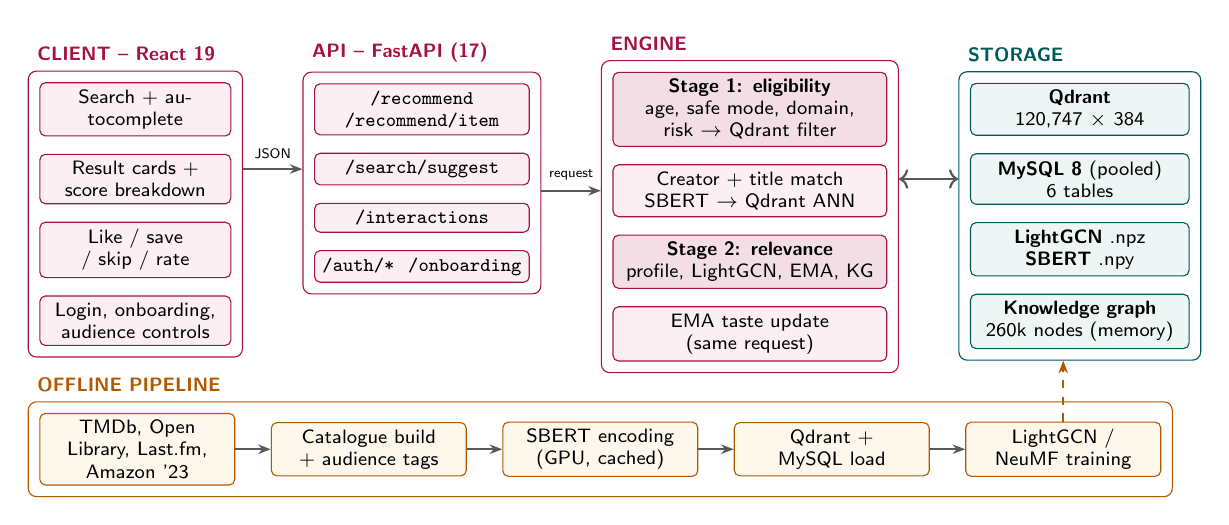
\begin{tikzpicture}[node distance=0.22cm]
        % Client
        \node[box, text width=2.25cm] (c1) {Search + autocomplete};
        \node[box, text width=2.25cm, below=of c1] (c2) {Result cards + score breakdown};
        \node[box, text width=2.25cm, below=of c2] (c3) {Like / save / skip / rate};
        \node[box, text width=2.25cm, below=of c3] (c4) {Login, onboarding, audience controls};
        \node[tier, fit=(c1)(c4), label={[lbl]north west:CLIENT \textendash{} React 19}] (client) {};
        % API
        \node[box, text width=2.55cm, right=1.05cm of c1] (a1) {\texttt{/recommend}\\ \texttt{/recommend/item}};
        \node[box, text width=2.55cm, below=of a1] (a2) {\texttt{/search/suggest}};
        \node[box, text width=2.55cm, below=of a2] (a3) {\texttt{/interactions}};
        \node[box, text width=2.55cm, below=of a3] (a4) {\texttt{/auth/*} \ \texttt{/onboarding}};
        \node[tier, fit=(a1)(a4), label={[lbl]north west:API \textendash{} FastAPI (17)}] (api) {};
        % Engine
        \node[box, text width=3.3cm, right=1.05cm of a1, fill=amritaMaroon!14] (e1) {\textbf{Stage 1: eligibility}\\ age, safe mode, domain, risk $\rightarrow$ Qdrant filter};
        \node[box, text width=3.3cm, below=of e1] (e2) {Creator + title match\\ SBERT $\rightarrow$ Qdrant ANN};
        \node[box, text width=3.3cm, below=of e2, fill=amritaMaroon!14] (e3) {\textbf{Stage 2: relevance}\\ profile, LightGCN, EMA, KG};
        \node[box, text width=3.3cm, below=of e3] (e4) {EMA taste update\\ (same request)};
        \node[tier, fit=(e1)(e4), label={[lbl]north west:ENGINE}] (eng) {};
        % Data
        \node[dbox, text width=2.6cm, right=1.05cm of e1] (d1) {\textbf{Qdrant}\\ 120,747 $\times$ 384};
        \node[dbox, text width=2.6cm, below=of d1] (d2) {\textbf{MySQL 8} (pooled)\\ 6 tables};
        \node[dbox, text width=2.6cm, below=of d2] (d3) {\textbf{LightGCN} .npz\\ \textbf{SBERT} .npy};
        \node[dbox, text width=2.6cm, below=of d3] (d4) {\textbf{Knowledge graph}\\ 260k nodes (memory)};
        \node[tier, draw=teal!70!black, fit=(d1)(d4), label={[lbl, text=teal!70!black]north west:STORAGE}] (data) {};
        % Arrows
        \draw[arr] (client.east |- a2) -- node[above, font=\sffamily\tiny]{JSON} (api.west |- a2);
        \draw[arr] (api.east |- e2) -- node[above, font=\sffamily\tiny]{request} (eng.west |- e2);
        \draw[arr, <->] (eng.east |- d2) -- (data.west |- d2);
        % Offline pipeline
        \node[obox, text width=2.3cm, below=0.85cm of c4.south west, anchor=north west] (o1) {TMDb, Open Library, Last.fm, Amazon '23};
        \node[obox, text width=2.3cm, right=0.45cm of o1] (o2) {Catalogue build + audience tags};
        \node[obox, text width=2.3cm, right=0.45cm of o2] (o3) {SBERT encoding (GPU, cached)};
        \node[obox, text width=2.3cm, right=0.45cm of o3] (o4) {Qdrant + MySQL load};
        \node[obox, text width=2.3cm, right=0.45cm of o4] (o5) {LightGCN / NeuMF training};
        \node[tier, draw=orange!70!black, fit=(o1)(o5), label={[lbl, text=orange!70!black]north west:OFFLINE PIPELINE}] (off) {};
        \draw[arr] (o1) -- (o2); \draw[arr] (o2) -- (o3); \draw[arr] (o3) -- (o4); \draw[arr] (o4) -- (o5);
        \draw[arr, dashed, draw=orange!70!black] (o5.north) -- (o5.north |- data.south);
    \end{tikzpicture}\end{adjustbox}

    \vspace{0.1cm}
    {\scriptsize Heavy objects (SBERT model, catalogue lookups, Qdrant client) load once at start-up; the API stays stateless per request.}
\end{frame}

\begin{frame}{2. Request Lifecycle: Eligibility, then Relevance}
    \framesubtitle{What happens between typing a query and seeing results}
    \centering
    \begin{adjustbox}{max width=\textwidth, max totalheight=0.60\textheight, center}
    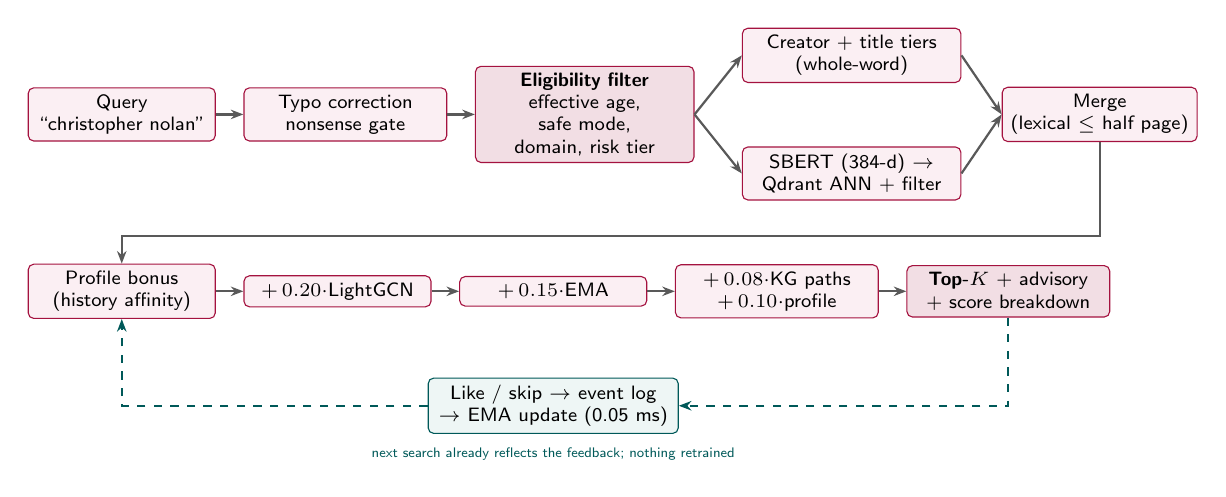
\begin{tikzpicture}[node distance=0.35cm]
        \node[box, text width=2.2cm] (q) {Query\\ ``christopher nolan''};
        \node[box, text width=2.4cm, right=of q] (t) {Typo correction\\ nonsense gate};
        \node[box, text width=2.6cm, right=of t, fill=amritaMaroon!14] (g) {\textbf{Eligibility filter}\\ effective age, safe mode,\\ domain, risk tier};
        \node[box, text width=2.6cm, right=0.6cm of g, yshift=0.75cm] (r1) {Creator + title tiers\\ (whole-word)};
        \node[box, text width=2.6cm, right=0.6cm of g, yshift=-0.75cm] (r2) {SBERT (384-d) $\rightarrow$\\ Qdrant ANN + filter};
        \node[box, text width=2.3cm, right=0.6cm of g, xshift=3.3cm] (m) {Merge\\ (lexical $\leq$ half page)};
        \draw[arr] (q) -- (t); \draw[arr] (t) -- (g);
        \draw[arr] (g.east) -- (r1.west); \draw[arr] (g.east) -- (r2.west);
        \draw[arr] (r1.east) -- (m.west); \draw[arr] (r2.east) -- (m.west);

        \node[box, text width=2.2cm, below=1.55cm of q] (s1) {Profile bonus\\ (history affinity)};
        \node[box, text width=2.2cm, right=of s1] (s2) {$+\,0.20\cdot$LightGCN};
        \node[box, text width=2.2cm, right=of s2] (s3) {$+\,0.15\cdot$EMA};
        \node[box, text width=2.4cm, right=of s3] (s4) {$+\,0.08\cdot$KG paths\\ $+\,0.10\cdot$profile};
        \node[box, text width=2.4cm, right=of s4, fill=amritaMaroon!14] (s5) {\textbf{Top-$K$} + advisory\\ + score breakdown};
        \draw[arr] (m.south) |- ($(s1.north)+(0,0.35)$) -- (s1.north);
        \draw[arr] (s1) -- (s2); \draw[arr] (s2) -- (s3); \draw[arr] (s3) -- (s4); \draw[arr] (s4) -- (s5);

        \node[dbox, text width=3.0cm, below=0.9cm of s3] (fb) {Like / skip $\rightarrow$ event log $\rightarrow$ EMA update (0.05 ms)};
        \draw[arr, dashed, draw=teal!70!black] (s5.south) |- (fb.east);
        \draw[arr, dashed, draw=teal!70!black] (fb.west) -| (s1.south);
        \node[font=\sffamily\tiny, text=teal!70!black, below=0.05cm of fb] {next search already reflects the feedback; nothing retrained};
    \end{tikzpicture}\end{adjustbox}

    \vspace{0.15cm}
    \begin{block}{Why this order}
        \scriptsize Ineligible items are removed \emph{before} anything is scored, so no reranker can promote them back. Fusion is additive, so the UI can show exactly how many points each signal added.
    \end{block}
\end{frame}

% =========================================================================
% SECTION 3: SUBSYSTEMS, DB & API
% =========================================================================
\begin{frame}{3. Subsystem Design: Database Schema}
    \framesubtitle{MySQL 8: six tables, idempotent migrations, shared connection pool}
    \centering
    \begin{adjustbox}{max width=\textwidth, max totalheight=0.52\textheight, center}
    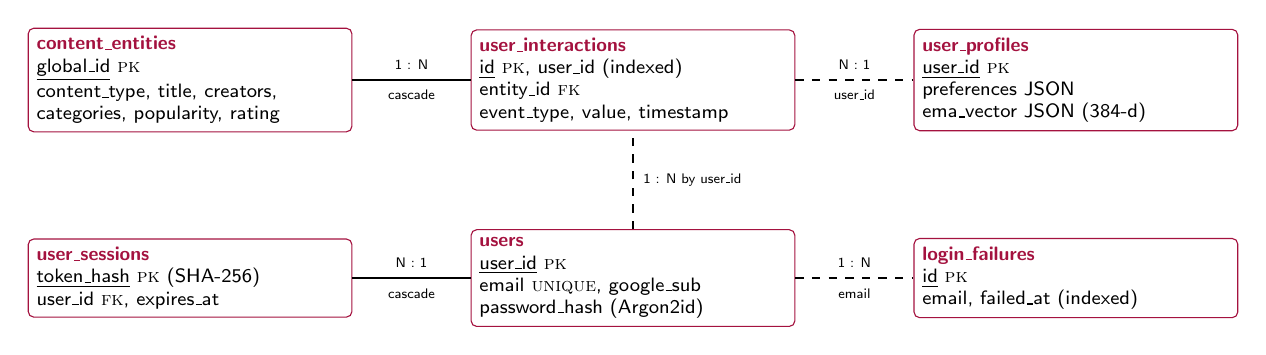
\begin{tikzpicture}
        \node[ent] (ce) {\textbf{\textcolor{amritaMaroon}{content\_entities}}\\ \underline{global\_id} \textsc{pk}\\ content\_type, title, creators,\\ categories, popularity, rating};
        \node[ent, right=1.5cm of ce] (ui) {\textbf{\textcolor{amritaMaroon}{user\_interactions}}\\ \underline{id} \textsc{pk}, user\_id (indexed)\\ entity\_id \textsc{fk}\\ event\_type, value, timestamp};
        \node[ent, right=1.5cm of ui] (up) {\textbf{\textcolor{amritaMaroon}{user\_profiles}}\\ \underline{user\_id} \textsc{pk}\\ preferences JSON\\ ema\_vector JSON (384-d)};
        \node[ent, below=1.25cm of ui] (us) {\textbf{\textcolor{amritaMaroon}{users}}\\ \underline{user\_id} \textsc{pk}\\ email \textsc{unique}, google\_sub\\ password\_hash (Argon2id)};
        \node[ent, left=1.5cm of us] (se) {\textbf{\textcolor{amritaMaroon}{user\_sessions}}\\ \underline{token\_hash} \textsc{pk} (SHA-256)\\ user\_id \textsc{fk}, expires\_at};
        \node[ent, right=1.5cm of us] (lf) {\textbf{\textcolor{amritaMaroon}{login\_failures}}\\ \underline{id} \textsc{pk}\\ email, failed\_at (indexed)};
        \draw[thick] (ce.east) -- node[above, font=\sffamily\tiny]{1 : N} node[below, font=\sffamily\tiny]{cascade} (ui.west);
        \draw[thick, dashed] (ui.east) -- node[above, font=\sffamily\tiny]{N : 1} node[below, font=\sffamily\tiny]{user\_id} (up.west);
        \draw[thick] (se.east) -- node[above, font=\sffamily\tiny]{N : 1} node[below, font=\sffamily\tiny]{cascade} (us.west);
        \draw[thick, dashed] (us.east) -- node[above, font=\sffamily\tiny]{1 : N} node[below, font=\sffamily\tiny]{email} (lf.west);
        \draw[thick, dashed] (us.north) -- node[right, font=\sffamily\tiny]{1 : N by user\_id} (ui.south);
    \end{tikzpicture}\end{adjustbox}

    \vspace{0.2cm}
    \begin{columns}[T]
        \column{0.48\textwidth}
        \begin{block}{Integrity}
            \scriptsize Foreign keys cascade (catalogue $\rightarrow$ events, users $\rightarrow$ sessions). Account deletion removes events, profile, sessions, lockout rows and the user in \textbf{one transaction}.
        \end{block}
        \column{0.48\textwidth}
        \begin{block}{Where the audience fields live}
            \scriptsize Domain, maturity, minimum age and risk tier are integer payload fields in \textbf{Qdrant}, where the eligibility filter runs during the search.
        \end{block}
    \end{columns}
\end{frame}

\begin{frame}{3. Subsystem Decomposition \& API Contracts}
    \framesubtitle{17 FastAPI endpoints, Pydantic-validated, documented live at \texttt{/docs}}
    \begin{columns}[T]
        \column{0.56\textwidth}
        \tiny
        \renewcommand{\arraystretch}{1.25}
        \begin{tabular}{L{2.25cm} L{5.15cm}}
            \toprule
            \textbf{Endpoint} & \textbf{Contract} \\
            \midrule
            \texttt{POST /recommend} & query, user\_id, age, safe\_mode, domain, top\_k $\rightarrow$ results with \texttt{score} + 6 per-signal scores, \texttt{match\_kind}, advisory, corrected query \\
            \texttt{POST /recommend/item} & ``more like this'', same eligibility gate \\
            \texttt{POST /interactions} & view, like, save, skip, done, rating $\rightarrow$ logged + EMA updated \\
            \texttt{/auth/*} & signup, login, Google, logout, me, delete; cookie session \\
            \texttt{GET /onboarding/items} & 22 starter picks, one per genre \\
            \midrule
            \multicolumn{2}{l}{\textbf{Errors:} 400 bad input $\cdot$ 401/403 access $\cdot$ 429 lockout $\cdot$ 503 dependency down} \\
            \bottomrule
        \end{tabular}
        \column{0.42\textwidth}
        \centering
        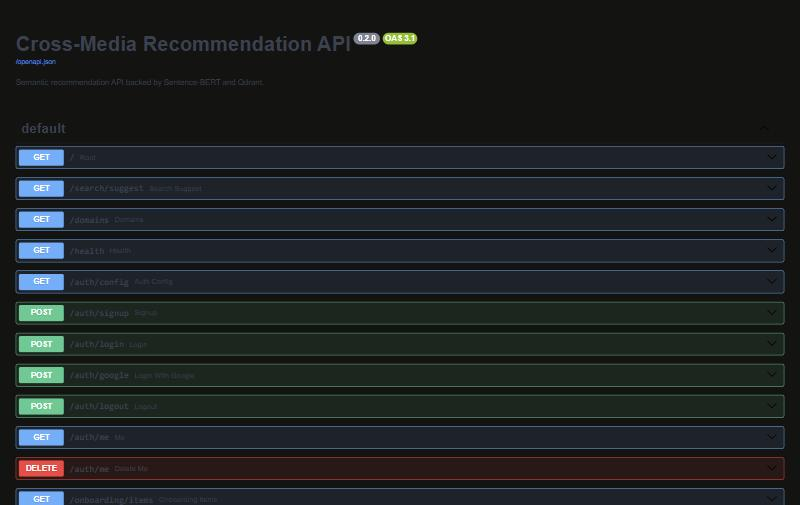
\includegraphics[width=\linewidth]{swagger_api.jpg}\\[1pt]
        {\tiny The running API's interactive documentation}
    \end{columns}
\end{frame}

% =========================================================================
% SECTION 4: IMPLEMENTATION
% =========================================================================
\section{Implementation Details}

\begin{frame}{4. Implementation Details -- Overview}
    \framesubtitle{Frontend, Backend, Database \& API Integration Status}
    \tiny
    \renewcommand{\arraystretch}{1.22}
    \begin{tabular}{L{2.5cm} L{8.9cm} c}
        \toprule
        \textbf{Layer / Subsystem} & \textbf{Completed Implementation} & \textbf{Status} \\
        \midrule
        Frontend & React 19 + Vite + Tailwind: 21 components, 3 pages; explainable result cards, audience controls, optimistic toggles & 100\% (Integrated) \\
        Data pipeline & 9 sources $\rightarrow$ one 20-column catalogue: 120,747 items, 7 content types, real TMDb age certificates & 100\% (Integrated) \\
        Recommendation engine & Hybrid retrieval, in-search eligibility, typed knowledge graph (260k nodes), 5-signal additive fusion, typo correction & 100\% (Integrated) \\
        Backend / API & FastAPI, 17 endpoints, dependency injection, consistent error mapping & 100\% (Integrated) \\
        Database & MySQL 8, 6 tables, idempotent migrations, cascade deletes, connection pool & 100\% (Integrated) \\
        Accounts \& security & Email + Google sign-in, sessions, lockout, onboarding, self-service deletion & 100\% (Functional) \\
        Models \& evaluation & LightGCN and NeuMF (PyTorch), 16-way ablation, latency and constraint studies. \textit{Open: dot-product LightGCN in the app, multi-seed runs} & 90\% (In progress) \\
        \bottomrule
    \end{tabular}

    \vspace{0.2cm}
    \begin{block}{Build, Deployment \& Version Control}
        \scriptsize
        \begin{itemize}
            \item \textbf{Deploy:} \texttt{scripts/demo\_up.ps1} checks MySQL, builds the client, starts the API, waits for \texttt{/health}, serves the build ( \texttt{-Public}: HTTPS tunnel, \texttt{-Stop}: shut down).
            \item \textbf{Repository:} \texttt{github.com/sanjay-pokee/Real-Time-Adaptive-Cross-Media-Recommendation-System} $\cdot$ GitHub Actions CI on every push.
        \end{itemize}
    \end{block}
\end{frame}

\begin{frame}{5. Core Subsystem: Data Pipeline \& Catalogue}
    \framesubtitle{Nine sources normalised into one schema, with audience labels}
    \begin{columns}[T]
        \column{0.47\textwidth}
        \scriptsize
        \renewcommand{\arraystretch}{1.15}
        \begin{tabular}{l l r}
            \toprule
            \textbf{Type} & \textbf{Source} & \textbf{Items} \\
            \midrule
            Movie & TMDb API & 23,492 \\
            Show & TMDb API & 10,617 \\
            Book & Open Library & 12,402 \\
            Music & Spotify CSV + Last.fm & 31,133 \\
            Health & Amazon Reviews 2023 & 20,000 \\
            Industrial & Amazon Reviews 2023 & 20,000 \\
            Finance & Amazon + Open Library & 3,103 \\
            \midrule
            \textbf{Total} & 4 domains & \textbf{120,747} \\
            \bottomrule
        \end{tabular}
        \column{0.51\textwidth}
        \begin{block}{Implementation}
            \scriptsize
            \begin{itemize}
                \item \textbf{Normalisers} per source write one 20-column schema; a new Amazon vertical is a config entry.
                \item \textbf{Audience tagging:} real TMDb US certificates for films (G $\rightarrow$ all ages, PG-13 $\rightarrow$ teen, R $\rightarrow$ adult); audited keyword rules elsewhere; unknown labels fail to the \emph{most} restrictive level.
                \item \textbf{Embeddings:} SBERT MiniLM, 384-d, re-encoded only when an item's text hash changes.
                \item \textbf{Fetchers} retry with back-off and resume after interruption.
            \end{itemize}
        \end{block}
    \end{columns}
\end{frame}

\begin{frame}{5. Core Subsystem: Retrieval \& Eligibility}
    \framesubtitle{Hybrid retrieval with the safety rule inside the vector query}
    \begin{columns}[T]
        \column{0.52\textwidth}
        \begin{block}{Hybrid retrieval}
            \scriptsize
            \begin{itemize}
                \item \textbf{Creator} (3 tiers) and \textbf{title} (5 tiers) whole-word matching: answers ``Christopher Nolan'' or ``F1'', where vectors fail.
                \item \textbf{Semantic:} SBERT query $\rightarrow$ Qdrant cosine search: answers intent such as ``space adventure with aliens''.
                \item \textbf{Typos} fixed from the catalogue's own vocabulary (``hary poter'' $\rightarrow$ ``harry potter''); a query with no catalogue word skips vector search.
            \end{itemize}
        \end{block}
        \begin{block}{Eligibility, fail-closed}
            \scriptsize
            \begin{itemize}
                \item No age given $\rightarrow$ teen ceiling; safe mode $\rightarrow$ child ceiling (7+).
                \item Compiled into Qdrant's \texttt{Filter(must=[...])}: an ineligible item is \textbf{never retrieved}.
            \end{itemize}
        \end{block}
        \column{0.46\textwidth}
        \centering
        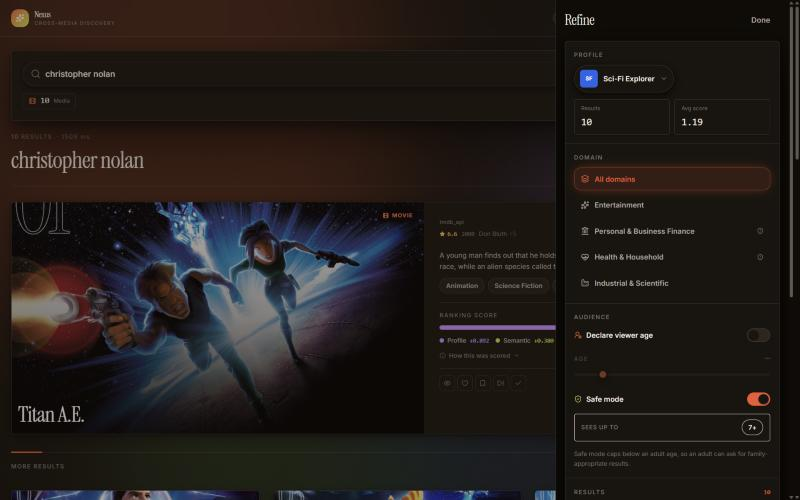
\includegraphics[width=\linewidth]{safe_mode.jpg}\\[1pt]
        {\tiny Safe mode on: ceiling 7+, every 13+ Nolan film removed before scoring}
    \end{columns}
\end{frame}

\begin{frame}{5. Core Subsystem: Personalisation \& Explainable Ranking}
    \framesubtitle{Five signals fused additively; adapts on every click without retraining}
    \begin{columns}[T]
        \column{0.52\textwidth}
        \scriptsize
        \[
          s = s_{\mathrm{ret}} + B_{\mathrm{pref}} + 0.20\,g + 0.15\,e + 0.08\,k + 0.10\,p
        \]
        \begin{itemize}
            \item $s_{\mathrm{ret}}$: cosine or match score; $B_{\mathrm{pref}}$: category affinity from history (liked $-0.15$, skipped $-0.35$).
            \item $g$: \textbf{LightGCN} (64-d, 3 layers, BPR) user--item similarity.
            \item $e$: \textbf{EMA taste vector}, updated per event:\\
            $\mathbf{v} \leftarrow \mathrm{norm}((1-\alpha w)\mathbf{v} + \alpha w(\pm\mathbf{x}_i))$, $\alpha=0.25$.
            \item $k$: knowledge-graph path score (next slide); $p$: declared-profile match.
            \item Toggles: a second click \emph{undoes} a like everywhere (EMA, profile, training log).
        \end{itemize}
        \column{0.46\textwidth}
        \centering
        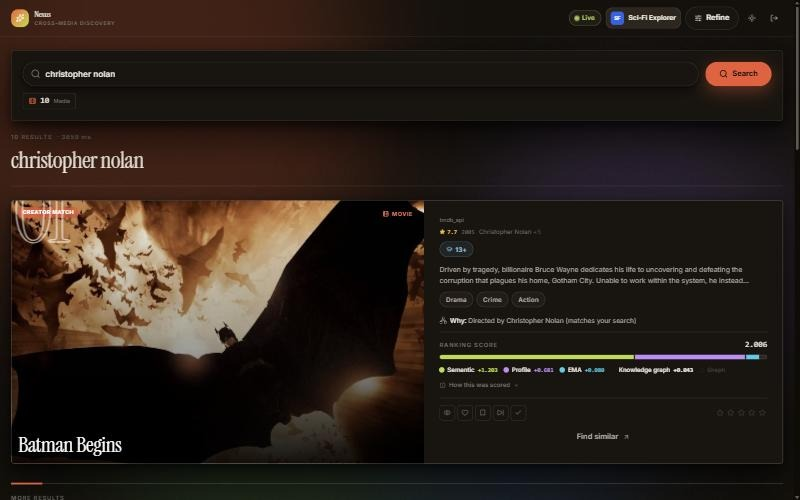
\includegraphics[width=\linewidth]{search_results_kg.jpg}\\[1pt]
        {\tiny Every card shows the points each signal added (Semantic +1.20, Profile +0.68, EMA +0.08, KG +0.04) and why}
    \end{columns}
\end{frame}

\begin{frame}{5. Core Subsystem: Knowledge Graph}
    \framesubtitle{Typed entity graph over the catalogue, scored by entity links and 2-hop paths}
    \begin{columns}[T]
        \column{0.50\textwidth}
        \centering
        \begin{adjustbox}{max width=\linewidth, max totalheight=0.60\textheight}
        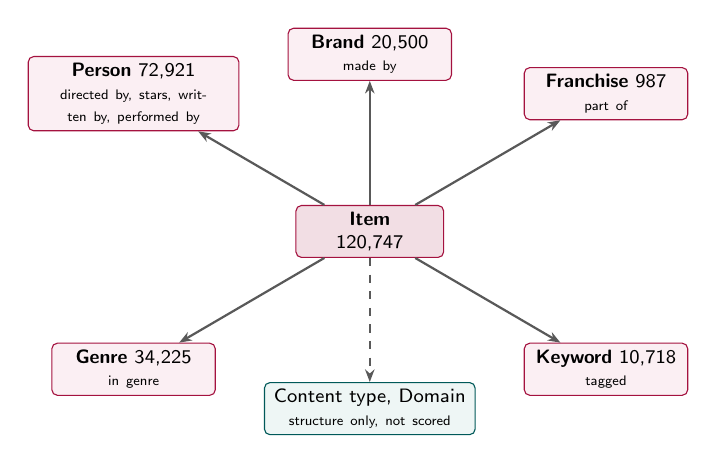
\begin{tikzpicture}
            \node[box, fill=amritaMaroon!14, text width=1.7cm] (item) at (0,0) {\textbf{Item}\\ 120,747};
            \node[box, text width=2.5cm] (person) at (-3.0,1.75) {\textbf{Person} 72,921\\ {\tiny directed by, stars, written by, performed by}};
            \node[box, text width=1.9cm] (brand) at (0,2.25) {\textbf{Brand} 20,500\\ {\tiny made by}};
            \node[box, text width=1.9cm] (franchise) at (3.0,1.75) {\textbf{Franchise} 987\\ {\tiny part of}};
            \node[box, text width=1.9cm] (genre) at (-3.0,-1.75) {\textbf{Genre} 34,225\\ {\tiny in genre}};
            \node[box, text width=1.9cm] (keyword) at (3.0,-1.75) {\textbf{Keyword} 10,718\\ {\tiny tagged}};
            \node[dbox, text width=2.5cm] (ctype) at (0,-2.25) {Content type, Domain\\ {\tiny structure only, not scored}};
            \foreach \n in {person, brand, franchise, genre, keyword} \draw[arr] (item) -- (\n);
            \draw[arr, dashed] (item) -- (ctype);
        \end{tikzpicture}
        \end{adjustbox}\\[3pt]
        {\tiny \textbf{260,109} nodes $\cdot$ \textbf{1,015,044} typed edges $\cdot$ built in $\sim$3 s $\cdot$ exported for Neo4j}
        \column{0.48\textwidth}
        \begin{block}{Scoring}
            \scriptsize
            \begin{itemize}
                \item \textbf{Entity linking:} query n-grams become nodes (``christopher nolan'' is one Person); items score by the share they connect to (IDF).
                \item \textbf{2-hop paths:} liked item $\rightarrow$ entity $\leftarrow$ candidate, a relation- and IDF-weighted cosine.
            \end{itemize}
        \end{block}
        \begin{block}{Example path (system output)}
            \centering
            \begin{adjustbox}{max width=\linewidth}
            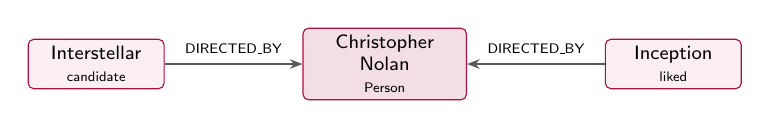
\begin{tikzpicture}
                \node[box, text width=1.55cm] (a) {Interstellar\\ {\tiny candidate}};
                \node[box, text width=1.9cm, right=1.75cm of a, fill=amritaMaroon!14] (b) {Christopher Nolan\\ {\tiny Person}};
                \node[box, text width=1.55cm, right=1.75cm of b] (c) {Inception\\ {\tiny liked}};
                \draw[arr] (a) -- node[above, font=\sffamily\tiny]{DIRECTED\_BY} (b);
                \draw[arr] (c) -- node[above, font=\sffamily\tiny]{DIRECTED\_BY} (b);
            \end{tikzpicture}
            \end{adjustbox}\\[3pt]
            {\scriptsize \textbf{Why:} \emph{Directed by Christopher Nolan, like Inception, which you liked}}
        \end{block}
    \end{columns}
\end{frame}

\begin{frame}{5. Core Subsystem: Accounts, Persistence \& Deployment}
    \framesubtitle{Service implementations, state management \& end-to-end wiring}
    \begin{columns}[T]
        \column{0.49\textwidth}
        \begin{block}{Accounts \& security}
            \scriptsize
            \begin{itemize}
                \item Email (Argon2id) or Google ID token, verified on the server.
                \item Random session token in an HttpOnly cookie; only its SHA-256 is stored.
                \item 5 wrong passwords $\rightarrow$ 15-minute lock, stored in MySQL so a restart does not lift it.
                \item An account's data needs that account's session (401 / 403).
                \item New accounts pick 22 starter items; deletion erases everything.
            \end{itemize}
        \end{block}
        \column{0.49\textwidth}
        \begin{block}{Persistence \& state}
            \scriptsize
            \begin{itemize}
                \item Shared pool of 10 connections: \textbf{3.9 ms vs 18 ms} per read; falls back to a direct connection under bursts.
                \item Like / skip $\rightarrow$ event row $\rightarrow$ EMA vector updated in the same request.
            \end{itemize}
        \end{block}
        \begin{block}{Deployment \& CI}
            \scriptsize
            \begin{itemize}
                \item One command builds and starts the stack, with health-check smoke tests.
                \item GitHub Actions: 390 tests on Windows, lint + build of the client on Linux.
            \end{itemize}
        \end{block}
    \end{columns}
\end{frame}

% =========================================================================
% SECTION 5: TESTING & DEMONSTRATION
% =========================================================================
\section{System Testing \& Demonstration}

\begin{frame}{6. System Testing \& Quality Verification}
    \framesubtitle{Unit, Integration, System Testing \& Quality Benchmarks}
    \scriptsize
    \renewcommand{\arraystretch}{1.2}
    \begin{tabular}{L{2.4cm} L{5.4cm} L{3.9cm} c}
        \toprule
        \textbf{Testing Level} & \textbf{Subsystems / Workflows Covered} & \textbf{Cases / Metrics} & \textbf{Status} \\
        \midrule
        Unit & Audience rules, eligibility, knowledge graph, LightGCN / NeuMF maths, EMA, typo correction, toggles & 390 automated tests in 19 files, $\sim$10 s & Passed \\
        Integration & API routes, Qdrant filter = Python rule, auth, lockout after restart, pool fallback & FastAPI TestClient with fakes & Passed \\
        System / E2E & Deployed stack in the browser; 17 live scenarios through the API & health-checked start-up & Passed \\
        Boundary \& error & Empty query, unknown domain, wrong password, unknown labels, internal error & 400 / 401 / 429; never unfiltered & Passed \\
        Regression in CI & Every push, clean machine, no data needed & GitHub Actions & Passed \\
        \bottomrule
    \end{tabular}

    \vspace{0.25cm}
    \begin{block}{System Stability \& Performance Summary}
        \scriptsize
        \begin{itemize}
            \item \textbf{Verification:} 390 / 390 tests pass locally and in CI; the browser walkthrough showed no console errors.
            \item \textbf{Performance:} Qdrant server: p50 \textbf{363 ms}, p95 \textbf{455 ms}; embedded (demo laptop) $\approx$1.8 s; KG $<$10 ms.
        \end{itemize}
    \end{block}
\end{frame}

\begin{frame}{6. Quality Benchmarks: Latency \& Audience Safety}
    \framesubtitle{Where the time goes, and whether the filter ever leaks}
    \begin{columns}[T]
        \column{0.46\textwidth}
        \begin{block}{Latency by stage (Qdrant server, 700 requests)}
            \scriptsize
            \renewcommand{\arraystretch}{1.12}
            \begin{tabular}{l r}
                \toprule
                Lexical match & 199 ms \\
                Qdrant ANN search & 85 ms \\
                Creator match & 46 ms \\
                Query encoding (SBERT) & 13 ms \\
                Profile + EMA + KG rerank & 26 ms \\
                LightGCN rerank & 0.07 ms \\
                \midrule
                \textbf{End to end (p95)} & \textbf{455 ms} \\
                Embedded Qdrant (demo laptop) & $\approx$1.8 s \\
                \bottomrule
            \end{tabular}
        \end{block}
        \column{0.52\textwidth}
        \begin{block}{Audience constraint evaluation (top 20)}
            \scriptsize
            \renewcommand{\arraystretch}{1.12}
            \begin{tabular}{l c c c}
                \toprule
                \textbf{Viewer} & \textbf{Sees} & \textbf{Filter on} & \textbf{Filter off} \\
                \midrule
                Child (8) & 4.1\% & \textbf{0.000} & 1.000 \\
                Teen (15) & 54.5\% & \textbf{0.000} & 1.000 \\
                No age given & 54.5\% & \textbf{0.000} & 1.000 \\
                Adult, safe mode & 4.1\% & \textbf{0.000} & 1.000 \\
                Adult (25) & 100\% & \textbf{0.000} & 0.000 \\
                \bottomrule
            \end{tabular}\\[2pt]
            {\tiny Violation rate = share of the top 20 the viewer may not see.}
        \end{block}
    \end{columns}
\end{frame}

\begin{frame}{6. Ranking Quality: NCF vs LightGCN (Panel Recommendation)}
    \framesubtitle{Amazon Reviews 2023, identical graphs and splits, leave-last-one-out, full-catalogue ranking, $K=20$}
    \centering
    \scriptsize
    \renewcommand{\arraystretch}{1.2}
    \begin{tabular}{l ccc ccc}
        \toprule
        & \multicolumn{3}{c}{\textbf{Movies \& TV} (50k users)} & \multicolumn{3}{c}{\textbf{Industrial \& Scientific} (34k users)} \\
        \cmidrule(lr){2-4}\cmidrule(lr){5-7}
        \textbf{Model} & R@20 & NDCG@20 & MRR@20 & R@20 & NDCG@20 & MRR@20 \\
        \midrule
        Popularity & 0.0182 & 0.0080 & 0.0052 & 0.0264 & 0.0111 & 0.0070 \\
        LightGCN, cosine (paper / app) & 0.0288 & 0.0125 & 0.0080 & 0.0326 & 0.0138 & 0.0087 \\
        NeuMF (NCF) & 0.0344 & 0.0138 & 0.0081 & 0.0416 & 0.0180 & 0.0115 \\
        \textbf{LightGCN, dot product} & \textbf{0.0454} & \textbf{0.0194} & \textbf{0.0121} & \textbf{0.0589} & \textbf{0.0254} & \textbf{0.0162} \\
        \bottomrule
    \end{tabular}

    \vspace{0.3cm}
    \begin{columns}[T]
        \column{0.48\textwidth}
        \begin{block}{Finding}
            \scriptsize NeuMF only wins against LightGCN scored by \emph{cosine}. Scored by the dot product it was trained with, LightGCN is \textbf{1.32$\times$ / 1.42$\times$} NeuMF: normalising threw away the popularity signal in vector length.
        \end{block}
        \column{0.48\textwidth}
        \begin{block}{Signal ablation (paper, 16 combinations)}
            \scriptsize Full hybrid is best on Movies \& TV (R@20 0.0368 vs 0.0197 popularity) and Industrial (0.0495 vs 0.0282); adding LightGCN to semantic search is the largest single gain.
        \end{block}
    \end{columns}
\end{frame}

\begin{frame}{7. System Demonstration \& Execution Walkthrough}
    \framesubtitle{Stable Live Execution, End-to-End Workflows \& Visual Outputs}
    \begin{columns}[T]
        \column{0.48\textwidth}
        \centering
        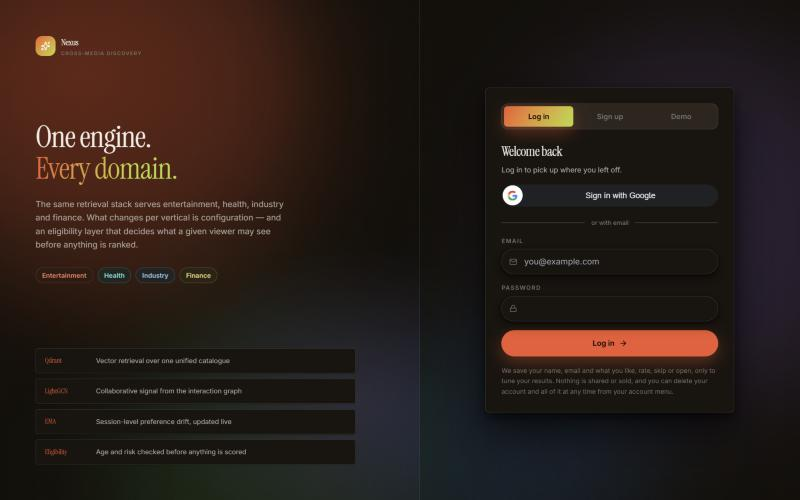
\includegraphics[width=0.8\linewidth]{login_page.jpg}\\[1pt]
        {\tiny Sign-in: email, Google or a demo profile, with a privacy notice}
        \column{0.48\textwidth}
        \centering
        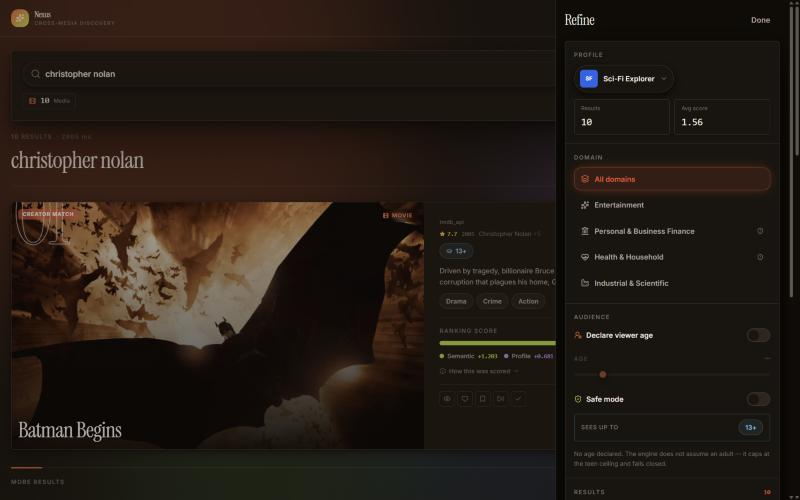
\includegraphics[width=0.8\linewidth]{refine_panel.jpg}\\[1pt]
        {\tiny Domain packs and audience controls (no age given $\rightarrow$ teen ceiling)}
    \end{columns}
    \vspace{0.15cm}

    \begin{block}{Live Demonstration Scenario}
        \scriptsize \textbf{1.} Start everything with \texttt{demo\_up.ps1} $\rightarrow$ \textbf{2.} sign in as a demo profile $\rightarrow$ \textbf{3.} search ``christopher nolan'': read the score breakdown and the knowledge-graph \emph{Why} $\rightarrow$ \textbf{4.} like three items and search again: the EMA share grows $\rightarrow$ \textbf{5.} turn on safe mode: every 13+ film disappears $\rightarrow$ \textbf{6.} switch to the Health domain: advisory banner $\rightarrow$ \textbf{7.} show \texttt{/docs} and the green CI run.
    \end{block}
\end{frame}

% =========================================================================
% SECTION 6: TECHNICAL KNOWLEDGE
% =========================================================================
\section{Technical Knowledge}

\begin{frame}{8. Software Engineering Decisions \& Technical Justification}
    \framesubtitle{Architecture Patterns, Concurrency, Security \& Maintainability}
    \begin{columns}[T]
        \column{0.48\textwidth}
        \begin{block}{1. Architectural \& Design Patterns}
            \scriptsize
            \begin{itemize}
                \item Layered tiers with dependency injection; handlers are tested with fakes.
                \item Eligibility-then-relevance pipeline; domains as configuration.
            \end{itemize}
        \end{block}
        \begin{block}{2. Data Integrity \& Concurrency}
            \scriptsize
            \begin{itemize}
                \item Cascading foreign keys, one-transaction deletion, chunked idempotent upserts.
                \item Pooled connections reset their session on return; known gap: EMA update is unlocked read-modify-write.
            \end{itemize}
        \end{block}
        \column{0.48\textwidth}
        \begin{block}{3. Security, Auth \& Validation}
            \scriptsize
            \begin{itemize}
                \item Argon2id, hashed session tokens, HttpOnly SameSite cookie, server-side Google verification.
                \item Persisted lockout; per-account access checks; Pydantic validation of every input.
            \end{itemize}
        \end{block}
        \begin{block}{4. Error Handling, Logging \& Scalability}
            \scriptsize
            \begin{itemize}
                \item Explicit 400 / 401 / 403 / 429 / 503; never an unfiltered fallback; per-run logs.
                \item Scale-out path: Qdrant as a server with payload indexes, MySQL replicas, stateless API workers.
            \end{itemize}
        \end{block}
    \end{columns}
\end{frame}

\begin{frame}{8. Model \& Design Choices}
    \framesubtitle{Why each component is what it is}
    \scriptsize
    \renewcommand{\arraystretch}{1.25}
    \begin{tabular}{L{2.7cm} L{3.4cm} L{6.4cm}}
        \toprule
        \textbf{Choice} & \textbf{Alternative} & \textbf{Reason} \\
        \midrule
        SBERT MiniLM-L6 (384-d) & Larger encoders & 13 ms per query keeps p95 under 500 ms; English-only is the accepted trade-off \\
        Filter \emph{inside} Qdrant & Filter after ranking & A post-filter can be undone by a reranker; this cannot leak (0.000) \\
        LightGCN in serving & NeuMF & Precomputed vectors, one dot product (0.07 ms); NeuMF needs a network pass per pair, and loses once LightGCN is scored by dot product \\
        EMA taste vector & Retraining & Session adaptation in 0.05 ms per event; LightGCN keeps long-term taste \\
        Additive fusion & Learned black box & Exact per-signal points in the UI and counterfactual re-ranking \\
        Hybrid lexical + vector & Vector only & Names and short titles (``F1'') carry no meaning for a vector \\
        Typed KG paths & Word overlap & Real entities (people, franchises) and an explainable 2-hop path; $<$10 ms \\
        \bottomrule
    \end{tabular}
\end{frame}

\begin{frame}{Limitations \& Future Scope}
    \framesubtitle{What is not done yet, stated plainly}
    \begin{columns}[T]
        \column{0.48\textwidth}
        \begin{block}{Current limitations}
            \scriptsize
            \begin{itemize}
                \item Single machine, embedded Qdrant; no permanent host or container yet. Catalogue frozen at 14 Sep 2026.
                \item Knowledge graph lives in memory; the Neo4j export is not served yet. Embedded Qdrant: $\approx$1.8 s per search.
                \item In-app LightGCN trained on 13 demo personas (no real users yet); served by cosine.
                \item Hand-set fusion weights; profile bonus can outweigh weak relevance.
                \item Book and music age labels are heuristics; no password reset.
            \end{itemize}
        \end{block}
        \column{0.48\textwidth}
        \begin{block}{Future scope}
            \scriptsize
            \begin{itemize}
                \item Serve LightGCN by a rescaled dot product (+58--81\% Recall@20 offline).
                \item Keep NeuMF as a pluggable collaborative signal; tune with several seeds.
                \item Serve the knowledge graph from Neo4j; learn relation weights.
                \item Docker images and cloud deployment; Qdrant as a server; weekly catalogue refresh.
                \item Learn fusion weights from real logs; multilingual encoder.
            \end{itemize}
        \end{block}
    \end{columns}
\end{frame}

\begin{frame}{Project Deliverables \& Technical Enrichment}
    \framesubtitle{Repository, publication and certifications}
    \scriptsize
    \renewcommand{\arraystretch}{1.1}
    \begin{tabular}{L{3.1cm} L{8.4cm} c}
        \toprule
        \textbf{Deliverable} & \textbf{Details} & \textbf{Status} \\
        \midrule
        Source code & GitHub repository with README, 390 tests and CI & Completed \\
        TEA 1: research paper & ``Real-Time Adaptive Cross-Media Recommendation Using Semantic Embeddings, Knowledge Graph Scoring, and Graph Collaborative Learning'', ICMLDE 2026 (Procedia Computer Science); presenting on 27 November 2026 & Accepted \\
        TEA 2, TEA 3 & -- & Not undertaken \\
        \midrule
        Sanjay A. K. & Recommender Systems: Evaluation and Metrics (Coursera, 15 h) & Completed \\
        Eswara Raj M. & Nearest Neighbor Collaborative Filtering (Coursera, 14 h) & Completed \\
        Aditya Vijay & Databases and SQL for Data Science with Python (Coursera, 20 h) & Completed \\
        Himaneesh Reddy J. & Recommendation Systems on Google Cloud (Skills Boost, 16 h) & Completed \\
        \bottomrule
    \end{tabular}
\end{frame}

% =========================================================================
% REFERENCES & THANK YOU
% =========================================================================
\section{References}
\nocite{ak2026crossmedia,he2020lightgcn,he2017ncf,rendle2020ncfmf,rendle2009bpr,reimers2019sbert,hou2024amazon,zang2022cross}
\begin{frame}{References}
    \tiny
    \setlength{\itemsep}{0pt}\setbeamertemplate{bibliography item}[text]
    \bibliographystyle{ieeetr}
    \bibliography{../ref}
\end{frame}

\begin{frame}
    \centering
    {\Huge \textbf{\textcolor{amritaMaroon}{Thank You}}} \\[0.4cm]
    {\large \textbf{Questions \& Viva Voce}}
\end{frame}

\end{document}
